\documentclass{article}
\def\pathToRoot{../../}\input{\pathToRoot headers/sharedHeader}

\newtheorem{lemma}{Lemma}
\newtheorem{proposition}{Proposition}
\newtheorem{theorem}{Theorem}
\newtheorem{corollary}{Corollary}
\theoremstyle{definition}
\newtheorem{definition}{Definition}
\newtheorem{example}{Example}

\usetikzlibrary{cd}

\begin{document}
\title{Functors \\ Maps between Categories}
\author{Felix Rech \and Dominik Wagner}
\maketitle

We want to define structure-preserving maps between categories.
Since the morphisms are the most interesting part of a category, such a map should not just operate on objects, but on morphisms too.
In order to preserve the structure, it has to map identity morphisms to identity morphisms and compositions of morphisms to compositions.
This is made precise in the following definition.

\begin{definition}
  Let $\cat A$ and $\cat B$ be categories. A \demph{functor} $F \from \cat A\to\cat B$ consists of
    \begin{itemize}
    \item a function
      \begin{align*}
        \ob(\cat A)\to\ob(\cat B),
      \end{align*}
      written as $A\mapsto F(A)$ and
    \item for all objects $A$ and $A'$, a function
      \begin{align*}
        \cat A(A,A')\to\cat B(F(A),F(A')),
      \end{align*}
      written as $f\mapsto F(f)$
    \end{itemize}
    such that the following axioms are satisfies:
    \begin{itemize}
    \item $F(1_A)=1_{F(A)}$ for all objects $A$ and
    \item $F(f'\of f)=F(f')\of F(f)$ for all morphisms $A\xrightarrow{f}A'\xrightarrow{f'}A''$.
    \end{itemize}
\end{definition}

The image of such a functor can be thought of as a \textit{shadow} of category $\cat{A}$ in $\cat{B}$.
Sometimes we call the first function \demph{action on paths} and the second function \demph{action on morphisms}.
The definition of functors turns the class of categories into a category itself.

\begin{definition}
  We define a category $\Cat$ with categories as elements and functors as morphisms.
  The identity morphism on an object is the functor that maps every object and every morphism to itself.
  The composition is defined by composition of both actions on objects and composition of both actions on morphisms.
\end{definition}

Let us look at some examples of functors.
We recommend to check the axioms yourself in order to verify that they indeed satisfy our definition.

\begin{example}
  We define a \demph{powerset functor} $\Set \xrightarrow{\mathcal{P}} \Set$ by
  \begin{align*}
    \mathcal{P}(A) &\coloneqq \{ X \mid X \subseteq A \} \\
    \mathcal{P}(f) &\coloneqq (\{x, y, \ldots\} \mapsto \{f(x), f(y), \ldots\})
  \end{align*}
  for all objects $A$ and $B$ and morphisms $A \xrightarrow{f} B$.
  In a similar way we can define a functor that maps a set $A$ to the set of lists or to the set of multisets with elements in $A$ or to many other types of collections.
  In all those cases the action on morphisms allows us to apply a function element-wise on a collection.
  If you have experience in functional programing, this may seem familiar to you.
\end{example}

In the next few examples we will talk about a very simple type of algebraic structure with a binary operation that we now define.

\begin{definition}
  A set $M$ is a \demph{monoid} if it has a binary operation ${}*{} \from M \times M \to M$ that satisfies the following axioms.
  \begin{description}
    \item [Associativity] $(x * y) * z = x * (y * z)$ for all $x, y, z \in M$.
    \item [Neutral element] There is an element $e \in M$ such that $e * x = x = x * e$ for all $x \in M$.
  \end{description}
\end{definition}

This is the same as the definition of \emph{groups} except that we do not require inverses.
Similar to homomorphisms on groups, we define homomorphisms on monoids.

\begin{definition}
  Given two monoids $M$ and $N$, a function $M \xrightarrow{f} N$ is a \demph{monoid homomorphism} if it satisfies the axioms
  \begin{itemize}
    \item $f(e) = e$
    \item $f(x * y) = f(x) * f(y)$
  \end{itemize}
  where we write $e$ for the neutral element in both monoids and $*$ for the binary operation in both monoids.
\end{definition}

You might already spot some similarity to the functoriality axioms.
We capture this in our next example.

\begin{example}
  There is a one-to-one correspondence between monoids and categories with one object.
  Elements of the monoid correspond to morphisms in the category and the binary operation is interpreted as composition of morphisms.
  With this interpretation, the functoriality axioms are the same as the axioms for monoid homomorphisms, which means that the homomorphisms between two groups are exactly the functors between the representing categories.
\end{example}

\begin{example}
  Monoids together with monoid homomorphisms form a category.
  We can define a functor from the category of monoids to $\Set$ that maps every monoid to its element set and every homomorphism to the undelying function.
  This functor maps into a category that is similar to its domain but with less structure on the objects.
  Hence one can say that the functor \emph{forgets} the monoid structure.
  This can be observed on many other functors as well.
  We call such functors \demph{forgetful}.
  Forgetfulness is an informal concept and depends on our interpretation of the category, but usually it is obvious if you should call a functor forgetful.
\end{example}

\begin{example}
  There is a functor from the category of commutative monoids to the category of general monoids which maps every object and every morphism to itself.
  It is injective on objects and on arrows, which means that we can always say, where a resulting object \textit{came from}.
  But we still call it \emph{forgetful} because it maps into a category where in general the objects have less structure.
\end{example}

We saw two examples of functors that forget structure, but there are also functors that do the opposite and create structure.
We will take a look at one of them.

\begin{example}
  Given a set $A$, we define the \demph{free monoid} $A^*$ over $A$ as the set of lists with elements in $A$.
  As binary operation we use the concatenation of lists and as neutral element the empty list.
  If we have a function $A \xrightarrow{f} B$ between sets then we can lift it to a monoid homomorphism $A^* \xrightarrow{f^*} B^*$ that applies $f$ pointwise on a list, i.e.\ $f^*([x, y, \ldots]) = [f(x), f(y), \ldots]$.
  This gives us a functor that maps a set to its free monoid and hence \emph{adds structure}.
  In general we call such a functor a \demph{free functor}.
\end{example}

Next, we consider a further example of a $\Set$-valued functor which, unlike the previous one, is not forgetful.
\begin{example}
  \label{ex:Mset}
  Let $\cat M$ be a category with a single object $M$, i.e.\ a monoid. Then, a functor $F\from\cat M\to\Set$ is a set $S=F(M)$ together with functions $F(m)\from S\to S$ for $m\from M\to M$ in $\cat M$. Hence, we can introduce the short-hand notation
  \begin{align*}
    m\cdot s=F(m)(s).
  \end{align*}
  The functorality axioms for $F$ state that
  \begin{align*}
    1_M\cdot s&=F(1_M)(s)=1_S(s)=s\\
    (m\of m')\cdot s&=F(m\of m')(s)=(F(m)\of F(m'))(s)=F(m)(F(m')(s))=m\cdot (m'\cdot s)
  \end{align*}
  for all $m,m'\from M\to M$ and $s\in S$.

  As a consequence, a functor from a one-object category, which correspond to a monoid $M$, to $\Set$ is essentially a \emph{left $M$-set}. (Recall that a left $M$-set for a monoid $M$ is a set $S$ together with a function
  \begin{align*}
    {} \cdot {} \from M\times S&\to S\\
    (m,s)&\mapsto m\cdot s
  \end{align*}
  such that $(m\of m')\cdot s=m\cdot (m'\cdot s)$ and $1_M\cdot s=s$ for all $m,m'\in M$ and $s\in S$.)
\end{example}

\section{Functors between Preorders}
Next, suppose that $\cat P$ and $\cat Q$ are preorders regarded as categories. A functor $F\from\cat P\to\cat Q$ is a mapping $\ob(\cat P)\to\ob(\cat Q)$ of the objects together with a function
\begin{align*}
  \cat P(P,P')\to\cat Q(F(P),F(P'))
\end{align*}
for each $P,P'\in\ob(\cat P)$. In the special case of preorders the latter function states that
\begin{align*}
  P\leq_\cat P P'\rightarrow F(P)\leq_\cat Q F(P')
\end{align*}
due to the fact that for each pair of objects in a preorder there is either exactly one arrow between them (denoting that the first is smaller than the second) or none at all (denoting incomparability). Hence, functors between preorders correspond to monotonically (increasing) functions.

A very natural question to ask is whether there is also a general category theoretic analogue to monotonically decreasing functions, i.e.\ functions $F\from\ob(\cat P)\to\ob(\cat Q)$ between preorders $\cat P$ and $\cat Q$ such that
\begin{align*}
  P\leq_\cat P P'\rightarrow F(P)\geq_\cat Q F(P')
\end{align*}
for each $P,P'\in\ob(\cat P)$. Again, this is exactly the same as to demand that for each $P,P'\in\ob(\cat P)$ there is a function
\begin{align*}
  \cat P(P,P')\to\cat Q(F(P'),F(P)).
\end{align*}
Since there is the unique arrow in $\cat P(P,P')$ if and only if $\cat P^\op(P',P)$ contains the unique arrow we see that this amounts to the same as having a function
\begin{align*}
  \cat P^\op(P',P)\to\cat Q(F(P'),F(P)),
\end{align*}
that is we need to reverse the direction of the arrows w.r.t. $\cat P$. Due to the fact that the additional functorality axioms are trivially satisfied for preorders, we see that monotone decreasing functors are exactly the same as functors
\begin{align*}
  F\from\cat P^\op\to\cat Q
\end{align*}
for the corresponding categories $\cat P$ and $\cat Q$.

Such ``operations'' that are essentially functors but reverse the direction of the arrows are going to play a prominent role in later chapters. Therefore, they have a special name:
\begin{definition}
  Let $\cat A$ and $\cat B$ be categories. A \demph{contravariant functor} from $\cat A$ to $\cat B$ is a functor $\cat A^\op\to\cat B$.
\end{definition}
\section{Dual Vector Spaces and Contravariant Representable Functors}
Next, we are going to look at the generalization of a construction from linear algebra which is used in the study of bilinear mappings amongst others and which can be regarded as a special contravariant functor. The general idea is that we analyze objects by analyzing the mappings into them.

Let $\mathbb K$ be a field. Given any two $\mathbb K$-vector spaces $V$ and $W$ there is the vector space
\begin{align*}
  \Hom(V,W)=\{f\from V\to W\mid f \text{ linear}\}
\end{align*}
of linear mappings between $V$ and $W$ where the vector space operations (addition and scalar multiplication) are defined pointwise. Therefore, for a fixed $\mathbb K$-vector space $W$, we can define a mapping
\begin{align*}
  V\mapsto H_W(V)=\Hom(V,W).
\end{align*}
It seems reasonable that we can extend this to a functor $H_W\from\Vect_{\mathbb K}\to\Vect_{\mathbb K}$. So let us check the details: We still have to define its action on linear maps $f\from V\to V'$, that is we have to define a linear mapping
\begin{align*}
  H_W(f)\from H_W(V)=\Hom(V,W)\to H_W(V')=\Hom(V',W)
\end{align*}
 that satisfies the axioms. To do so, let $g\in H_W(V)=\Hom(V,W)$ be arbitrary and we have to come up with a linear mapping $V'\to W$. This seems to be impossible: There is no canonical way to construct a linear mapping $V'\to W$ from linear mappings $f\from V\to V'$ and $g\from V\to W$. Hence, there is no reasonable way to define a functor $H_W\from\Vect_{\mathbb K}\to\Vect_{\mathbb K}$.

However, it is perfectly possible to canonically construct a linear mapping $V\to W$ from linear mappings $f\from V\to V'$ and $g\from V'\to W$ by just taking its composition $g\of f$ (since composition preserves linearity):
\begin{align*}
  \xymatrix{V' \ar[r]^{f} & V \ar[r]^{g} & W }.
\end{align*}
That is, given arbitrary $f\from V\to V'$ we can define a mapping
\begin{align*}
  H_W(f)\from H_W(V')&\to H_W(V)\\
  g&\mapsto g\of f
\end{align*}
that is moreover trivially linear. This is looks like a contravariant functor. To verify that it is indeed a functor we check the axioms:
\begin{align*}
  H_W(1_V)&=\lambda g\ldotp g\of 1_V=\lambda g\ldotp g=1_{H_W(V)}\\
  H_W(f'\of f)=\lambda g\ldotp g\of (f'\of f)&=\lambda g\ldotp (g\of f')\of f=(\lambda g\ldotp g\of f)\of (\lambda g\ldotp g\of f')=H_W(f)\of H_W(f').
\end{align*}
Thus, we have defined a functor $H_W\from\Vect_{\mathbb K}^\op\to\Vect_{\mathbb K}$.

In linear algebra one frequently takes $\mathbb K$ itself for $W$ (regarded as a one-dimensional vector space over itself) and $H_{\mathbb K}(V)$ is called the dual vector space $V^*$ of $V$. It is a well known fact that the dual vector space $V^*$ reveals a lot about $V$ itself and its relation to other vector spaces. In particular, $V$ is a subspace of the dual of $V^*$.

Since this construction seems very useful indeed for vector spaces it is a natural question whether we can do something similar for arbitrary categories.
The obvious analogue to
\begin{align*}
  H_W(V)=\Hom(V,W)=\{f\from V\to W\mid f \text{ linear}\},
\end{align*}
 that is its effect on objects, is
\begin{align*}
  H_B(A)=\cat A(A,B)
\end{align*}
for $A,B\in\ob(\cat A)$. In contrast to the special case of vector spaces, $\cat A(A,B)$ is not a category again but just a collection. If all collections $\cat A(A,B)$ are sets this suggests a functor $F_A\from\cat A^\op\to\Set$. However, obviously this is only well-defined if all collections $\cat A(A,B)$ are really sets, which is not necessarily the case for arbitrary categories. Hence, in all what follows we assume a \emph{locally small} category $\cat A$ in which all collections $\cat A(A,B)$ are indeed sets.

Bearing this in mind, the defintion of the functor $H_B$ for $B\in\cat A$ is a straight-forward generalization:
\begin{align*}
  H_B(A)=\cat A(A,B)
\end{align*}
for objects $A\in\cat A$ and for $f\from A'\to A$ the function $H_B(f)\from H_B(A)\to H_B(A')$ is defined by
\begin{align*}
  H_B(f)\from H_B(A)=\cat A(A,B)&\to H_B(A')=\cat A(A',B)\\
  g&\mapsto g\of f.
\end{align*}
\vspace{-0.7cm}
\begin{align*}
  \xymatrix{A' \ar[r]^{f} & A \ar[r]^{g} & B }
\end{align*}
The functor $H_A$ is called the \emph{contravariant representable functor} of $A$. Furthermore, contravariant functors to $\Set$ (like $H_A$) have a special name:
\begin{definition}
  Let $\cat A$ be a category. A \demph{presheaf} on $\cat A$ is a functor $\cat A^\op\to\Set$.
\end{definition}
In a later chapter we are going to discover that contravariant representable functors really help us understand the structure of locally small categories. In particular, we are going to prove that two objects $A$ and $B$ are isomorphic if and only if $H_A$ and $H_B$ are isomorphic\footnote{The notion of mappings between functors is defined in the next chapter.}, i.e. $A$ and $B$ ``look the same from all other objects''.

\begin{example}
  Similarly, as in example \ref{ex:Mset} presheaves on one-object categories (i.e.\ monoids $M$) correspond to \emph{right} $M$-sets, where a right $M$-set is a set $S$ together with a function
  \begin{align*}
    {} \cdot {} \from S\times M&\to S\\
    (s,m)&\mapsto s\cdot m
  \end{align*}
  such that $s\cdot (m\of m')=(s\cdot m)\cdot m'$ and $s\cdot 1_M=s$ for all $m,m'\in M$ and $s\in S$.
\end{example}


\section{Full and Faithful functors}

The following definition introduces a concept that is similar to injectivity of functors but restricts only the action on morphisms, not on objects.

\begin{definition}
  A functor $\cat{A} \xrightarrow{F} \cat{B}$ is \demph{faithful} if for all objects $A, B \in \cat{A}$ the function
  \begin{align*}
    \cat{A}(A, B) &\to \cat{B}(F(A), F(B)) \\
    f &\mapsto F(f)
  \end{align*}
  is \emph{injective}.
\end{definition}

Note that this definition only speaks about what happens to morphisms between the \emph{same pair} of objects.
We can still map two different morphisms onto the same target, as long as they are defined between a different pair of objects.
Let us illustrate this with an example.
\[ 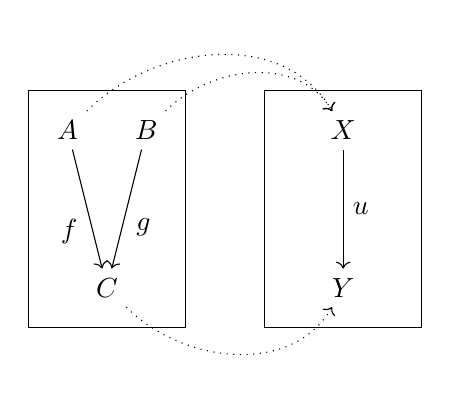
\begin{tikzpicture}
    \draw (0, 0) rectangle (2, 3);
    \node (A) at (0.5, 2.5) {$A$};
    \node (C) at (1, 0.5) {$C$};
    \node (B) at (1.5, 2.5) {$B$};
    \draw[->] (A) to node[auto, swap] {$f$} (C);
    \draw[->] (B) to node[auto] {$g$} (C);

    \draw (3, 0) rectangle (5, 3);
    \node (X) at (4, 2.5) {$X$};
    \node (Y) at (4, 0.5) {$Y$};
    \draw[->] (X) to node[auto] {$u$} (Y);

    \draw[->, dotted, out=45, in=120] (A) to (X);
    \draw[->, dotted, out=45, in=120] (B) to (X);
    \draw[->, dotted, out=-45, in=-120] (C) to (Y);
  \end{tikzpicture} \]
Assume that a functor $F$ is given by the dotted arrows and maps the morphism $f$ and $g$ both to $u$.
The functor is faithful nevertheless because the morphisms $f$ and $g$ start from different objects.

Analogously to the definition of faithfulness, we define fullness of a functor, which is similar to the concept of surjectivity.

\begin{definition}
  A functor $\cat{A} \xrightarrow{F} \cat{B}$ is \demph{full} if for all objects $A, B \in \cat{A}$ the function
  \begin{align*}
    \cat{A}(A, B) &\to \cat{B}(F(A), F(B)) \\
    f &\mapsto F(f)
  \end{align*}
  is \emph{surjective}.
\end{definition}


\section{Subcategories}

With the definition of full and faithful functors we adapted two set theoretic concepts for our work with categories.
The same can be done with the subset relation.
This time there is one obvious way to do it which is the following definition.

\begin{definition}
  Given two categories $\cat{A}$ and $\cat{B}$, we say that $\cat{A}$ is a \demph{subcategory} of $\cat{B}$ if $\ob(\cat{A}) \subseteq \ob(\cat{B})$ and for all objects $A, B \in \cat{A}$, we have the inclusion $\cat{A}(A, B) \subseteq \cat{B}(A, B)$.
\end{definition}

If we consider the inclusion functor $\cat{A} \to \cat{B}$ that maps every object and every morphism to itself, we can ask the question, whether it is full or faithful.
The faithfulness is obvious, but only certain subcategories have full inclusion functors.
This motivates the definition of full subcategories.

\begin{definition}
  A subcategory $\cat{A}$ of a category $\cat{B}$ is \demph{full} if for all objects $A, B \in \cat{A}$, there is an equality $\cat{A}(A, B) = \cat{B}(A, B)$, not just an inclusion.
\end{definition}

With our definition, a subcategory is full if and only if the inclusion functor is full.
A convenient property is that a full subcategory is completely determined by the selection of objects that it contains.

As the image of a monoid homomorphism is a monoid and the image of a group homomorphism is a group, one could easily assume that the image of a functor is a category, but in general this is wrong as we can see in the next example:
\[ \begin{tikzpicture}
  \draw (0, 0) rectangle (3, 5);
  \node (A) at (1, 4.5) {$A$};
  \node (B) at (1, 2.5) {$B$};
  \node (C) at (2, 2.5) {$C$};
  \node (D) at (2, 0.5) {$D$};
  \draw[->] (A) to node[auto] {$f$} (B);
  \draw[->] (C) to node[auto] {$g$} (D);

  \draw (4, 0) rectangle (7, 5);
  \node (X) at (5, 4.5) {$X$};
  \node (Y) at (5, 2.5) {$Y$};
  \node (Z) at (5, 0.5) {$Z$};
  \draw[->] (X) to node[auto] {$u$} (Y);
  \draw[->] (Y) to node[auto] {$v$} (Z);
  \draw[->, bend left=45] (X) to node[auto] {$v \of u$} (Z);

  \draw[->, dotted, in=120, out=45] (A) to (X);
  \draw[->, dotted, in=120, out=45] (B) to (Y);
  \draw[->, dotted, in=-120, out=-45] (C) to (Y);
  \draw[->, dotted, in=-120, out=-45] (D) to (Z);
\end{tikzpicture} \]
Assume that a functor $F$ is given by the dotted arrows and maps the morphism $f$ to $u$ and $g$ to $v$.
Since the image of $F$ contains $u$ and $v$, it should also contain $v \of u$ to be a category.
But $F$ does not map any morphism to $v \of u$, thus the image is not a category.

\end{document}

% vim mode line:
% vim: ts=2 sts=2 sw=2 expandtab
